\documentclass{article}
    \usepackage{url}
    \usepackage[margin=1.0in]{geometry}
    \usepackage{cite}
    \usepackage{amssymb}
    \usepackage{enumerate}
    \usepackage{enumitem}
    \usepackage{graphicx}
    \usepackage{xcolor}
    \usepackage{pdfpages}
    \usepackage{hyperref}
    \usepackage{listings}
    \usepackage{fancybox}
    \usepackage{lstautogobble}
    \usepackage{titling}
    \usepackage{pdflscape}
    \usepackage[nottoc,notlot,notlof]{tocbibind}
    \renewcommand\maketitlehooka{\null\mbox{}\vfill}
    \renewcommand\maketitlehookd{\vfill\null}

    \graphicspath{ {Resources/} }
    \title{ESP8266 Interface with DHT11 Sensor}
    \author{
        Jay Rovacsek
        \texttt{c3146220@uon.edu.au}\\
    }
    \date{\today}
    \hypersetup{
    colorlinks=true,
    linkcolor=black,
    filecolor=magenta,      
    urlcolor=blue,
    citecolor=red,
    linktoc=section,
    }
    \pagenumbering{arabic}

    \lstset{frame=tb,
        language=c++,
        aboveskip=2mm,
        belowskip=2mm,
        showstringspaces=false,
        columns=flexible,
        basicstyle={\small\ttfamily},
        numbers=none,
        numberstyle=\tiny\color{gray},
        keywordstyle=\color{blue},
        commentstyle=\color{dkgreen},
        stringstyle=\color{mauve},
        breaklines=true,
        breakatwhitespace=true,
        tabsize=3
    }

    \begin{document}

    \begin{titlingpage}
        \maketitle
    \end{titlingpage}
    \newpage
    
    \section{Outline}
    The proposed INFT3970 mjaor project required POC code for displaying and interfacing
    with a temperature sensor, in the following document and code the below units were used:
    \begin{itemize}
        \item ESP8266 NodeMCU unit \cite{ESP8266-EBAY}
        \item DHT11 Sensor Bundle \cite{DHT11-JAYCAR}
    \end{itemize}
    Code associated with this document used the datapin: D1, interfaced as:
    \begin{lstlisting}
        dht.setup(5, DHTesp::DHT11);
    \end{lstlisting}

    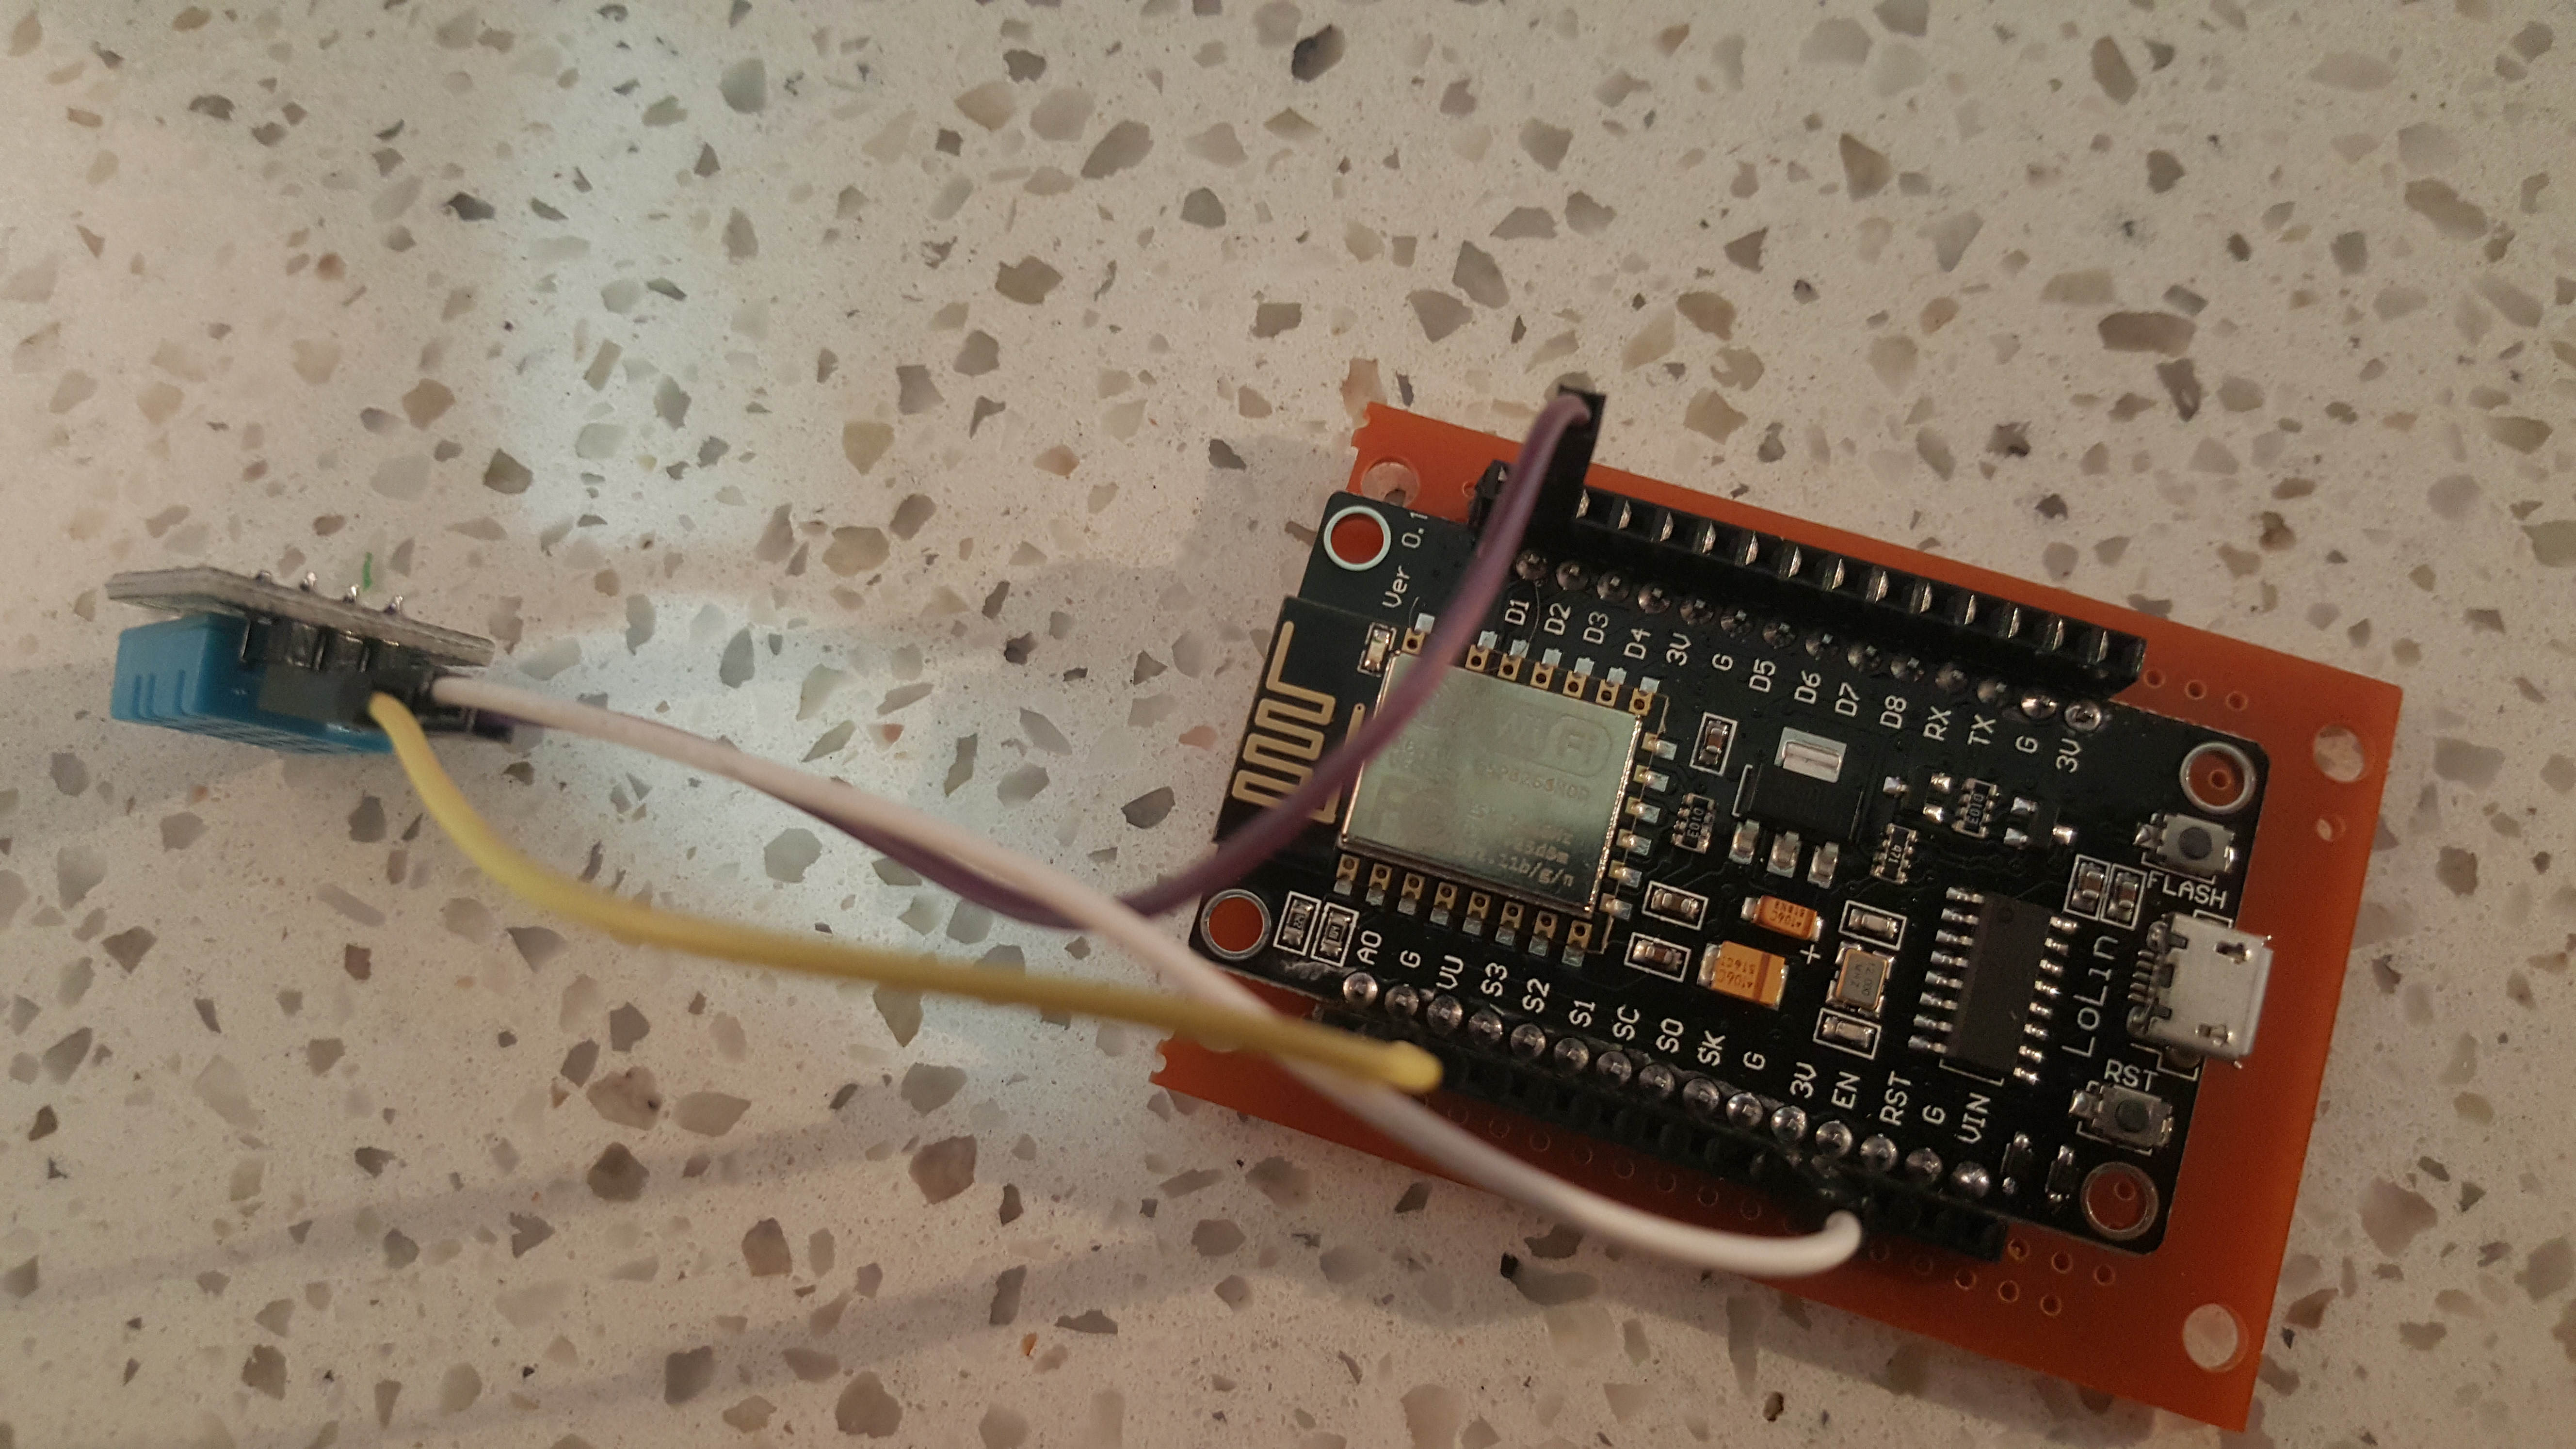
\includegraphics[width=\textwidth]{hardware-setup.jpg}

    \section{To Do}
    A number of changes are still required to interface correctly with a base
    ASP.NET MVC application \cite{Main-Project}, including the implementation of either:
    \begin{itemize}
        \item A RESTful API
        \item Sending of data to a predefined location within code.
    \end{itemize}

    Optimally we would implement a service setting behind a namespace accessible on the WAN as to best serve auto-association of devices with the correct service and avoid hardcoding many details beyond the FQDN.

    \newpage

    \begin{thebibliography}{9}
        \raggedright
        \bibitem{ESP8266-EBAY}
            \url{https://www.ebay.com.au/itm/New-NodeMcu-Lua-ESP8266-ESP-12E-CH340G-WIFI-Network-Development-Board-Module/162466934890}
        \bibitem{DHT11-JAYCAR}
            \url{https://www.jaycar.com.au/arduino-compatible-temperature-and-humidity-sensor-module/p/XC4520}
        \bibitem{Main-Project}
            \url{https://github.com/JayRovacsek/INFT3970}
    \end{thebibliography}

    \end{document}  
